\documentclass[	
  noindent
]{elteikthesis}[2024/04/26]
\usepackage{amsmath}
\usepackage{graphicx}
\usepackage{enumitem}

\begin{document}

\documentlang{hungarian}

\begin{titlepage}
  \centering
  \vspace*{3cm}
  {\Huge\bfseries Hálózati algoritmusok \par}
  {\Huge\bfseries Vizsgálati napló \par}
  
  \vspace{1cm} % Elválasztó vonal előtt egy kis tér
  \rule{0.8\linewidth}{0.5mm} % Elválasztó vonal
  
  \vspace{1cm} % Elválasztó vonal után egy kis tér
  {\large\bfseries Téma: 5. Reconfiguration and Locomotion with Joint Movements in the Amoebot Model \par} % Még kisebb betűméret
  
  \vspace{6cm}
  {\Large Kiss Marcell, Sándor Balázs, Varga Dávid István  \par}
  \vspace{1cm}
  {\large 2025.05.06. \par}
  \vfill
  {
\includegraphics[width=0.2\textwidth]{images/elte_cimer_szines.eps}\par}
\end{titlepage}


\tableofcontents

\chapter{Amoebot Szimuláció}
Ez a projekt egy amőba-szerű robotok (Amoebot) szimulációját valósítja meg az Eötvös Loránd Tudományegyetem Informatikai Karának MSc képzése keretében. A szimuláció célja a robotok viselkedésének és interakcióinak modellezése különböző színtereken.

\section{Általános ismertető}

A szimuláció Pygame-re épül, és lehetővé teszi az amőbotok különböző viselkedési mintáinak tesztelését különböző színtereken. A főmenüből választhatók ki a színterek, amelyek különböző elrendezéseket és kihívásokat kínálnak a robotok számára.

A main.py fájl inicializálja a Pygame-et, létrehozza a Simulation objektumot, és elindítja a fő ciklust, amely kezeli az eseményeket, frissíti az állapotokat, és megjeleníti a grafikát.

A Scene osztály felelős a különböző színterek beállításáért, míg a SceneLibrary osztály lehetővé teszi a színterek külön fájlban történő kezelését, elősegítve a kód modularizálását és karbantartását.

  \section{A program felépítése és elérhetősége}
    Az alábbiakban ismertetem a program elérhetőségét és mappaszerkezetét.

    \subsection{A program elérhetősége}
      A projekt GitHub repository-ja:
      \\
      \url{https://github.com/SandorBalazsHU/elte-ik-msc-amoebot}

    \subsection*{Mappastruktúra}
      A projekt mappaszerkezete az alábbi:
      \begin{verbatim}
        elte-ik-msc-amoebot/
        |-- src/
        |   |-- amoebot.py        - Az amobotok modellje
        |   |-- behaviors.py      - A megvalósított viselkedések gyűjteménye
        |   |-- config.py         - A konfigurációs változók gyűjteménye
        |   |-- drawer.py         - A rajzelemeket leíró osztály
        |   |-- menu_button.py    - A menüelemek gyűjteménye
        |   |-- scene.py          - A színtérkezelő
        |   |-- scene_library.py  - A megvalósított színterek gyűjteménye
        |   |-- simulation.py     - A szimulátor főosztály
        |   \-- triangle_map.py   - A háromszögrácsot és a foglaltságot kezelő osztály
        \-- main.py               - A főprogram
        \end{verbatim}

    \subsection{Használat}

      Telepítés: Győződj meg róla, hogy a szükséges függőségek telepítve vannak (pl. pygame, pygame_menu).
      
      Futtatás: A szimuláció elindításához futtasd a main.py fájlt:
      
      python main.py
      
      Navigáció: Használd a menüt a különböző színterek kiválasztásához és a szimuláció beállításához.
  
  \section*{Főbb osztályok és funkciók}
    Tekintsük most át a projekt főbb osztályait és funkcióit.

    \subsection*{Amoebot (amoebot.py)}
    Az \texttt{Amoebot} osztály reprezentálja az egyes robotokat a szimulációban. Főbb jellemzői:
    \begin{itemize}[left=0pt]
        \item \textbf{Állapotkezelés}: Aktív vagy passzív állapot.
        \item \textbf{Viselkedés}: Különböző viselkedési minták beállítása.
        \item \textbf{Mozgás}: A háromszög térképen való mozgás és kapcsolódás más robotokhoz.
    \end{itemize}
  
    \subsection*{Behavior (behaviors.py)}
    A \texttt{Behavior} osztály és a hozzá tartozó \texttt{BehaviorType} enumeráció különböző viselkedési mintákat definiál az amőbotok számára, például:
    \begin{itemize}[left=0pt]
        \item \textbf{RANDOM}: Véletlenszerű mozgás.
        \item \textbf{TO\_HEADING}: Meghatározott irányba való mozgás.
        \item \textbf{INTELLIGENT}: Intelligens viselkedés, például középpont keresése vagy cikcakk mozgás.
    \end{itemize}
  
    \subsection*{Scene (scene.py)}
    A \texttt{Scene} osztály kezeli a különböző színtereket a szimulációban. Főbb funkciói:
    \begin{itemize}[left=0pt]
        \item \textbf{Menükezelés}: Főmenü és beállítások menü megjelenítése.
        \item \textbf{Színterek beállítása}: Különböző színterek inicializálása, például véletlenszerű elrendezés, falak, meta-modulok.
    \end{itemize}
  
    \subsection*{SceneLibrary (scene\_library.py)}
    A \texttt{SceneLibrary} osztály célja a színterek külön fájlban történő tárolása és kezelése. Ez lehetővé teszi a \texttt{Scene} osztály karbantartásának egyszerűsítését és a kód modularizálását.
  
    \subsection*{TriangleMap (triangle\_map.py)}
    A \texttt{TriangleMap} osztály reprezentálja a háromszög alapú térképet, amelyen az amőbotok mozognak. Főbb funkciói:
    \begin{itemize}[left=0pt]
        \item \textbf{Pozíciókezelés}: Ellenőrzi, hogy egy adott pozíció foglalt-e.
        \item \textbf{Mozgás}: Lehetővé teszi az amőbotok számára a mozgást a térképen.
    \end{itemize}

    \section{Az Amőbot modell}
    Az amőbótot modellező szimuláció célja az egyes amőbák mozgásának és interakcióinak modellezése egy rácsos világban. Az amőbák különböző viselkedéseket követhetnek, és reagálhatnak környezetükre, azaz egymás helyére léphetnek, ütközhetnek, és meghatározott szabályok alapján csoportosulhatnak.
    
    A következő dokumentumban az amőbótot modellező rendszer felépítését és működését írjuk le, részletesen ismertetve annak működését és a Python programozási nyelven történő implementálását.
    
    \section{Amőbótot Modell: Elmélet}
    Az amőbák szimulációja egy klasszikus rácsos környezetben történik, ahol a világot egy mátrix vagy rács reprezentálja. Az amőbák az ezen rácsokhoz rendelt koordináták alapján mozognak, és képesek kölcsönhatásba lépni egymással, mint például ütközések elkerülése vagy pozíciók feloldása.
    
    Az amőbák **állapotok** és **viselkedési típusok** szerint működnek. Minden amőba tartalmazza a következőket:
    \begin{itemize}
        \item \textbf{Pozíció} – Az amőba aktuális koordinátái a rácsban.
        \item \textbf{Viselkedés} – Az amőba által végzett tevékenység, mint például véletlenszerű mozgás vagy koordinált csoportosulás.
        \item \textbf{Lépésszámláló} – Minden amőbának van egy lépésszámlálója, amely nyomon követi, hogy hány lépést tett meg. Ez befolyásolhatja a pozíció felszabadítását és egyéb műveleteket.
    \end{itemize}
    
    A viselkedés típusok között szerepelhet például:
    \begin{itemize}
        \item **Véletlenszerű mozgás** – Az amőba egy véletlen irányba lép.
        \item **Célzott mozgás** – Az amőba egy konkrét irányba mozog.
        \item **Intelligens viselkedés** – Az amőba alkalmazkodik a környezetéhez, például a középpont felé tart.
    \end{itemize}
    
    \section{Megvalósítás}
    A rendszer Pythonban van implementálva, és az amőbák osztálya a következő kulcsfontosságú attribútumokkal rendelkezik:
    
    \subsection{Amoebot Osztály}
    Az amőbák működését az \texttt{Amoebot} osztály valósítja meg. Az osztály tartalmazza a szükséges attribútumokat, mint például a pozíció, viselkedés, és a lépésszámláló.
    
    \begin{verbatim}
    class Amoebot:
        def __init__(self, triangle_map, row, col):
            self.triangle_map = triangle_map
            self.row = row
            self.col = col
            self.step_counter = 0
            self.from_pos = None
            self.behavior = None
            self.state = AmoebotState.PASSIVE
            # További inicializálás...
    \end{verbatim}
    
    \subsubsection{Lépéskezelés}
    Minden amőbának van egy \texttt{update} metódusa, amely kezeli a mozgását. Az amőba a \texttt{can\_move\_somewhere} logikát követi, hogy eldöntse, vajon képes-e mozogni a következő lépésben. Ha igen, elmenti a jelenlegi pozícióját a \texttt{from\_pos} változóba, majd kiszámolja az új célpontot és végrehajtja a mozgást.
    
    \begin{verbatim}
    def update(self):
        if self.can_move_somewhere():  # Ha lehetséges lépni
            self.from_pos = (self.row, self.col)
            new_row, new_col = self.calculate_target()
            self.row = new_row
            self.col = new_col
            self.triangle_map.occupy(new_row, new_col, self)
            self.step_counter += 1
            return True
        return False
    \end{verbatim}
    
    A \texttt{step\_counter} változó nyomon követi az amőba lépéseit. Minden második lépésnél a pozíció felszabadítása történik meg.
    
    \subsubsection{Pozíció felszabadítása}
    A pozíció felszabadítása akkor történik meg, ha az amőba elérte a szükséges lépésszámot, és ha a \texttt{Config.Scene.replace\_pos} beállítás engedélyezi ezt. A következő kód segít abban, hogy minden második lépésnél feloldjuk az előző helyet:
    
    \begin{verbatim}
    if self.step_counter % 2 == 0:
        if self.from_pos:
            self.triangle_map.release(*self.from_pos)
            self.from_pos = None
    \end{verbatim}
    
    \subsection{TriangleMap Osztály}
    Az amőbák mozgása a \texttt{TriangleMap} osztály segítségével történik, amely kezeli a rácsot, a helyek lefoglalását, és a pozíciók felszabadítását. Az amőbák csak akkor léphetnek, ha a célpontjuk üres, és ha az \texttt{occupy} metódus nem foglalja el a helyet.
    
    \begin{verbatim}
    class TriangleMap:
        def __init__(self):
            self.grid = [[None for _ in range(cols)] for _ in range(rows)]
    
        def occupy(self, row, col, amoebot):
            if self.grid[row][col] is None:
                self.grid[row][col] = amoebot
                return True
            return False
    
        def release(self, row, col):
            self.grid[row][col] = None
    \end{verbatim}
    
    \subsection{Viselkedés és Állapotok}
    Az amőbák különböző viselkedéseket képesek végrehajtani, például véletlenszerű mozgást vagy célzott mozgást. Az \texttt{AmoebotState} és a \texttt{BehaviorType} osztályok biztosítják, hogy az amőbák állapota és viselkedése változhasson, például amikor egy amőba eléri a célját vagy új viselkedést kell alkalmaznia.
    
    \begin{verbatim}
    class AmoebotState(Enum):
        PASSIVE = auto()
        ACTIVE = auto()
        MOVING = auto()
    
    class BehaviorType(Enum):
        RANDOM = auto()
        TO_HEADING = auto()
        INTELLIGENT = auto()
    \end{verbatim}
    
    \section{Összegzés}
    A szimuláció során az amőbák a rácsos világban mozognak, és különböző viselkedéseket alkalmaznak. Az amőbák mozgása és interakciói jól definiált szabályok szerint történnek, figyelembe véve a lépésszámlálást, pozíciók felszabadítását és a viselkedés típusokat. Az implementáció rugalmasan bővíthető további viselkedésekkel és interakciókkal.
    
\chapter{Szimulációk}
    Ebbena  fejezetben ismertetjük a szimulátor használatát és a megvalósított szimulációkat és méréseket
    \section{A menük}
      Most ismerjük meg a menürendszert.

      \subsection{A főmenü}
        A program indítása utána  főmenü fogad minket.

        \begin{figure}[H]
          \centering
          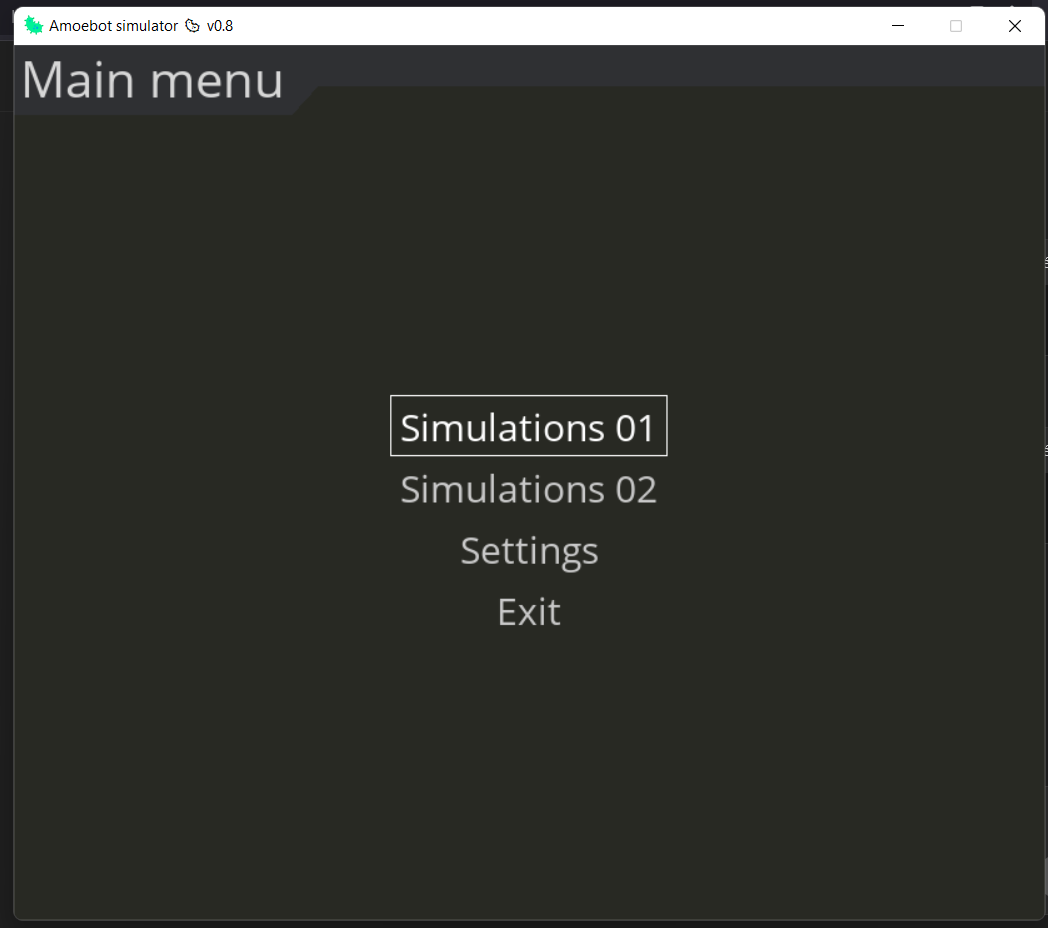
\includegraphics[width=0.6\textwidth]{images/simulatons/main_menu.png}
          \caption{A főmenü}
          \label{fig:main_menu}
        \end{figure}

        \subsection{A Simulation 01}
        A ebben a menüben érhetőek el az egyszerűbb szimulácik a szimulátor bemutatására.

        \begin{figure}[H]
          \centering
          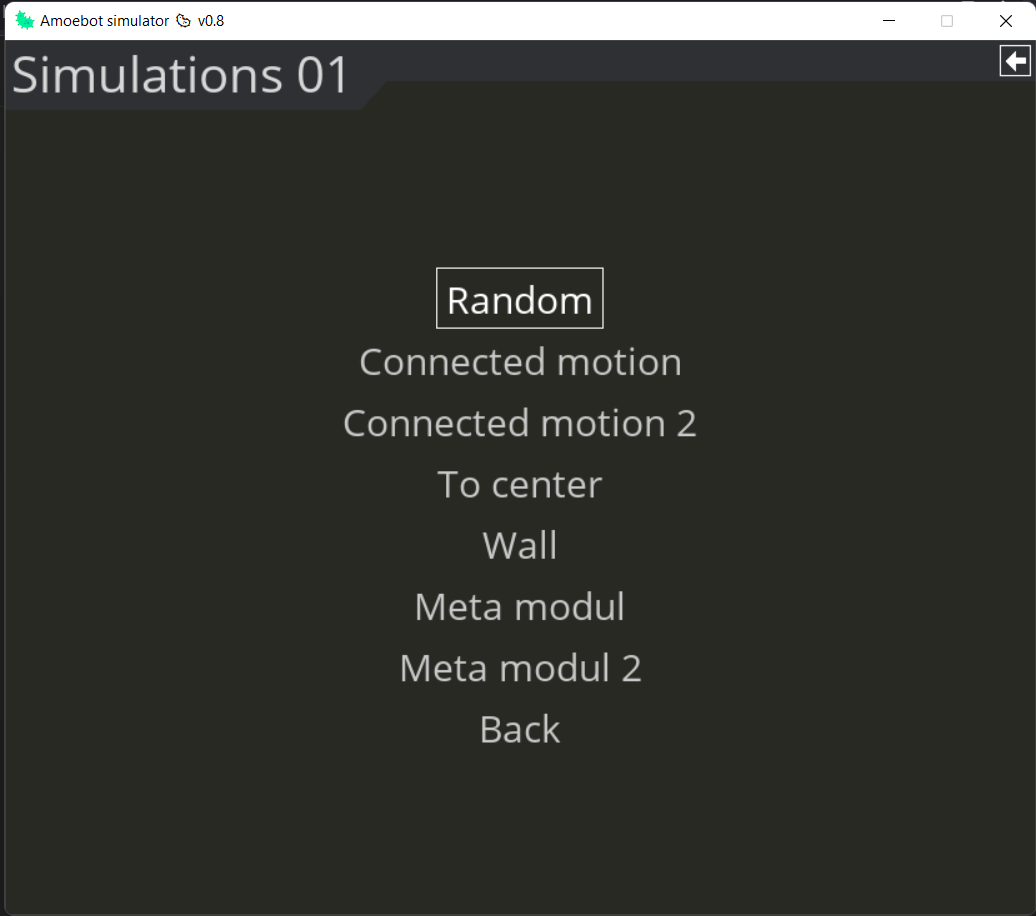
\includegraphics[width=0.6\textwidth]{images/simulatons/Simulation01.png}
          \caption{A Simulation 01 menü}
          \label{fig:Simulation01}
        \end{figure}

        \subsection{A Simulation 01}
        A ebben a menüben érhetőek el az összetettebb szimulácik.

        \begin{figure}[H]
          \centering
          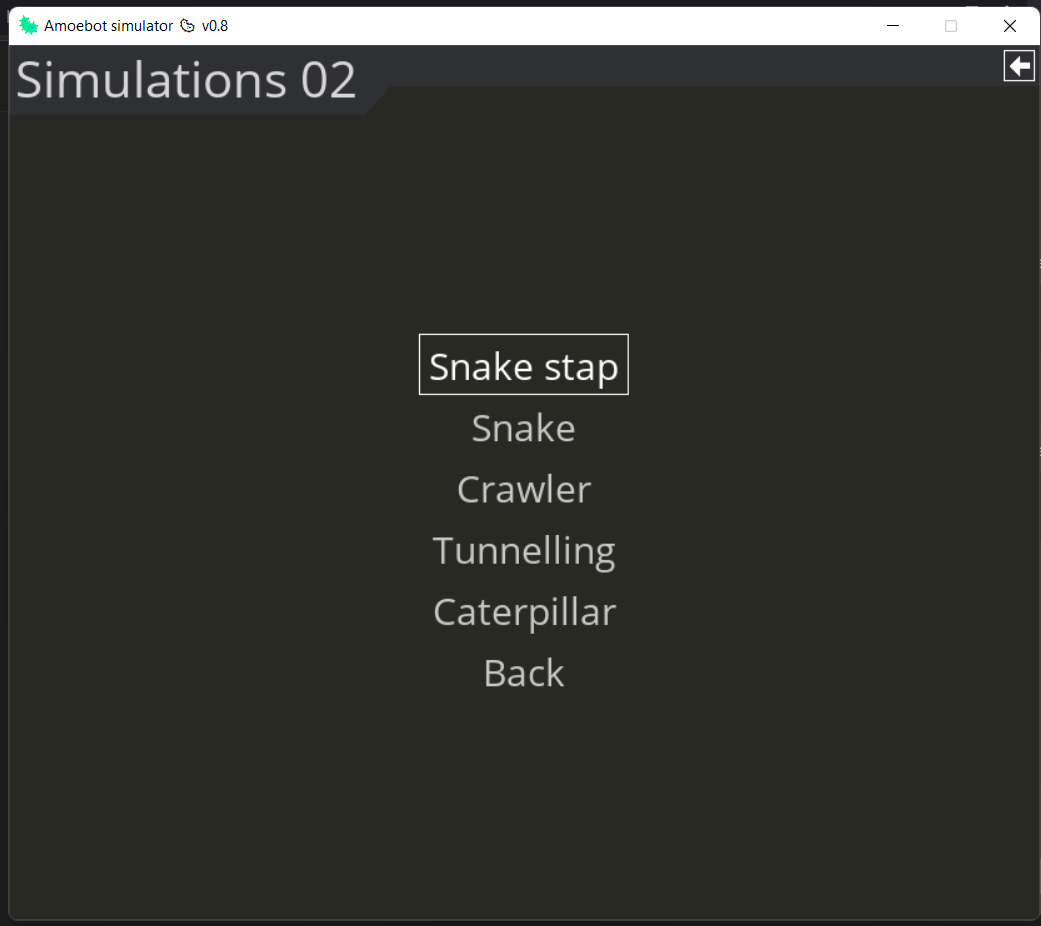
\includegraphics[width=0.6\textwidth]{images/simulatons/Simulation02.png}
          \caption{A Simulation 02 menü}
          \label{fig:Simulation01}
        \end{figure}

        \subsection{A Settings menü}
        A ebben a menüben érhetőek el a szimulátor beállításai.

        \begin{figure}[H]
          \centering
          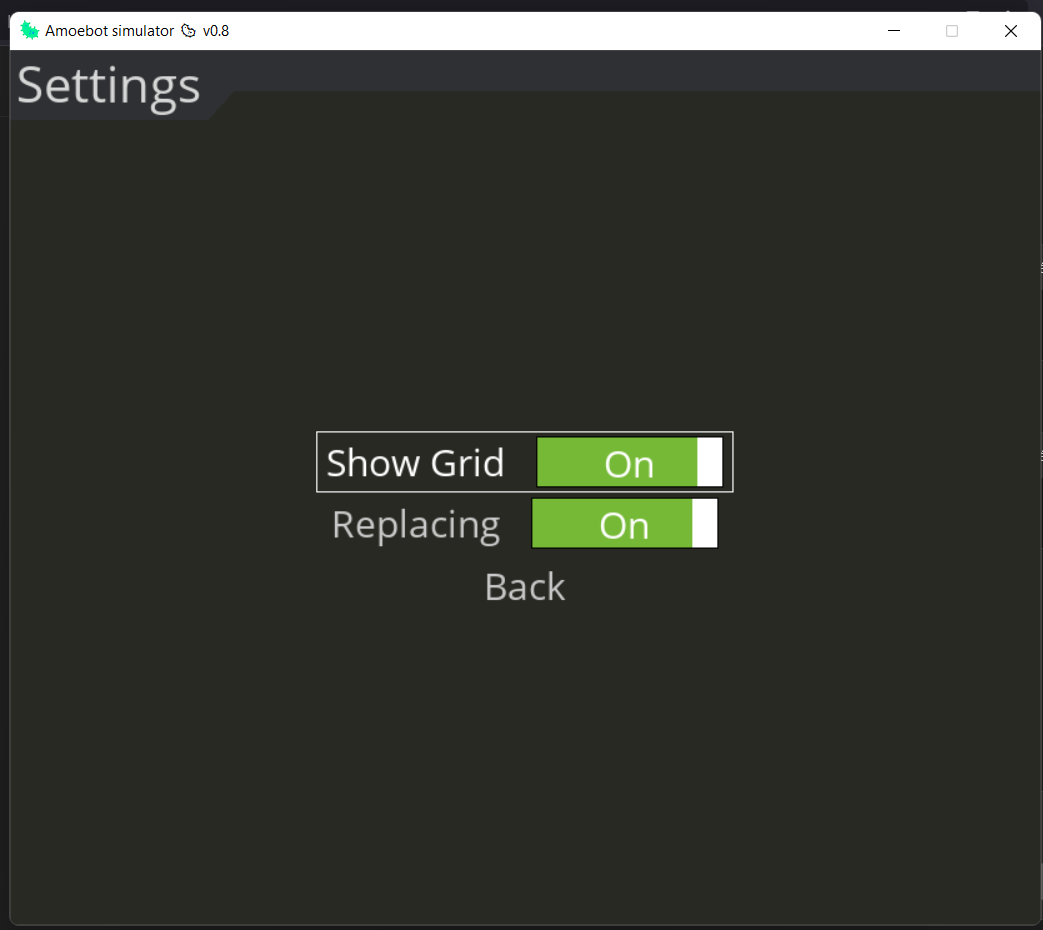
\includegraphics[width=0.6\textwidth]{images/simulatons/settings.png}
          \caption{A Simulation 02 menü}
          \label{fig:settings}
        \end{figure}

      \subsection{A Simulation 01 - Az egyszerűbb szimulációk}

\chapter{Mérések és eredményeik}
  Tekintsük át az elvégzett méréseket és eredményeit.

  \section{Mérési eredmények}
    \begin{table}[h!]
      \centering
      \begin{tabular}{|l|c|c|}
      \hline
      \textbf{Mozgásforma} & \textbf{Lépésszám} & \textbf{Maximális lépésszám} \\
      \hline
      Kígyó mozgás (hagyományos modell) & 14 & 9 \\
      Kígyó mozgás (fejlesztett modell) & 9 & 9 \\
      Lánctalp mozgás & 97 & 97 \\
      Lépegető mozgás & 9 & 9 \\
      \hline
      \end{tabular}
      \caption{Amőbot szimulációs eredmények különböző mozgásformák esetén}
      \label{tab:amobot_eredmenyek}
      \end{table}
  
      \begin{figure}[H]
        \centering
        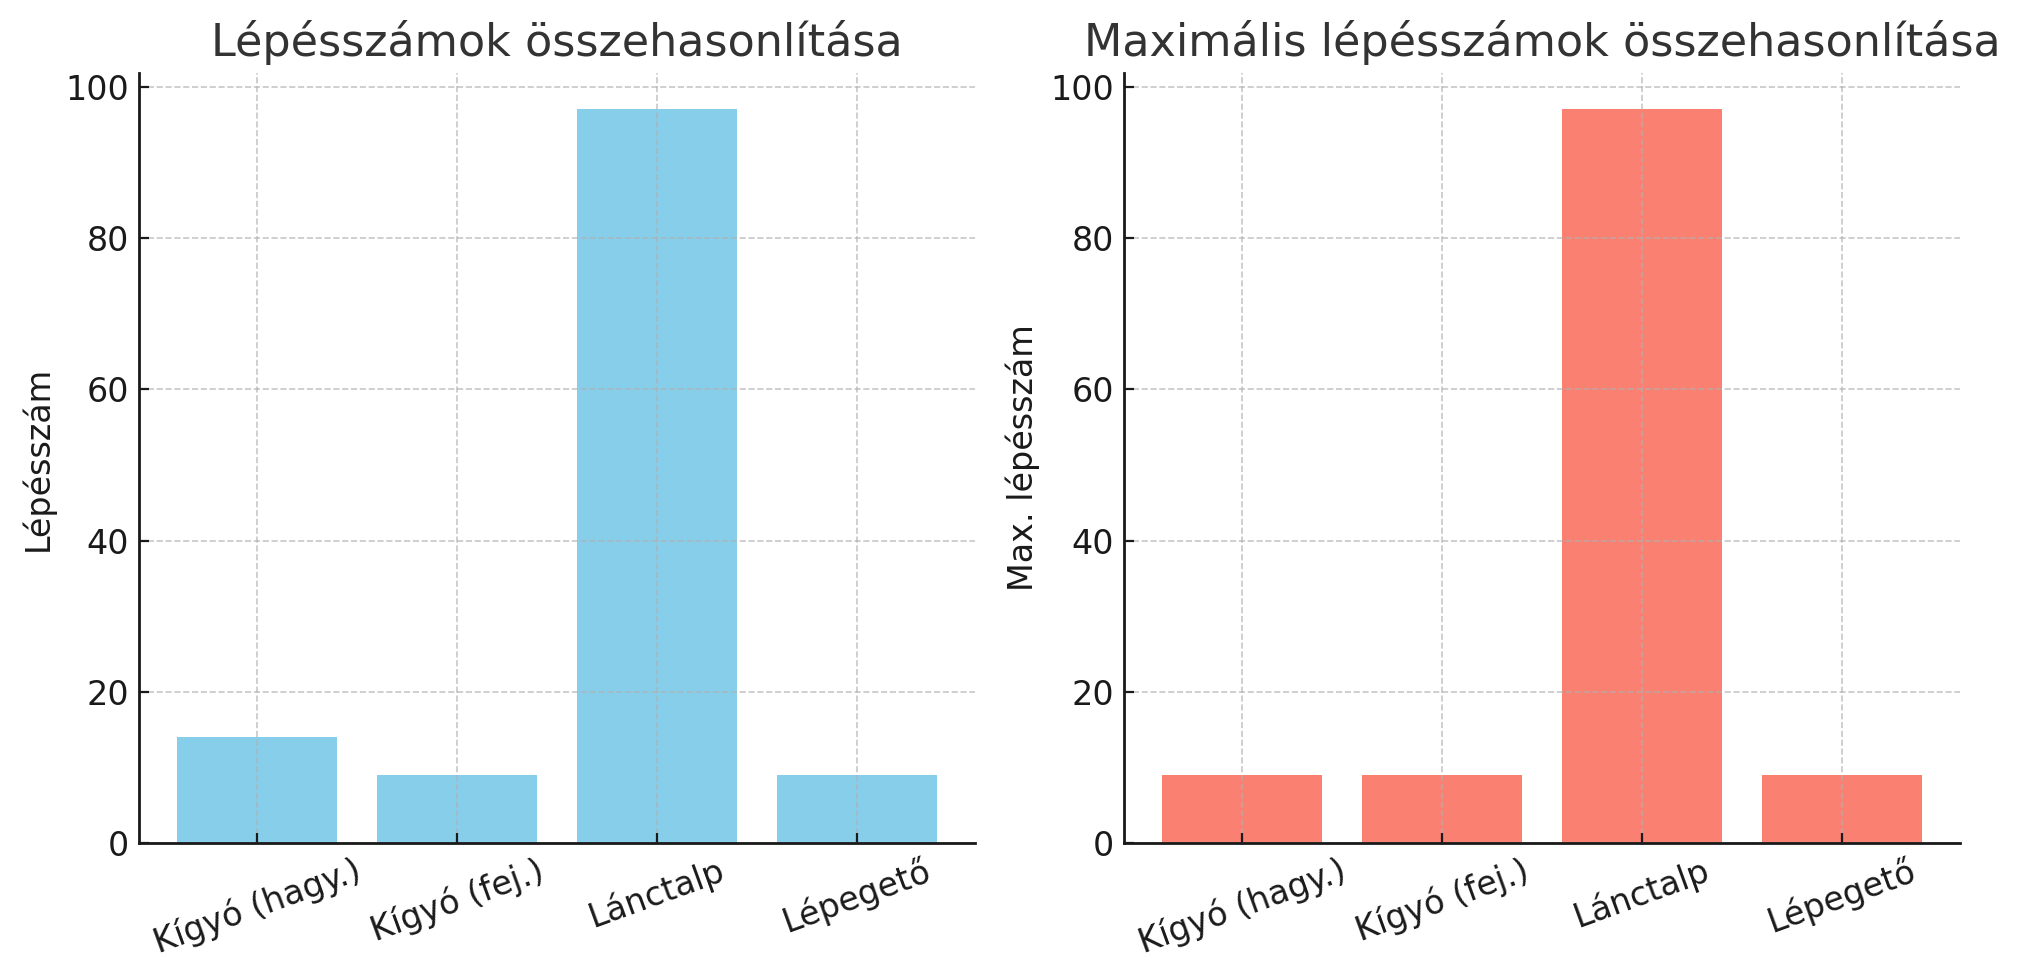
\includegraphics[width=1.0\textwidth]{images/mesurements/stat.png}
        \caption{A szimulációs statisztikák}
        \label{fig:stat}
      \end{figure}

\end{document}